\documentclass{beamer}

\usepackage{préambule}

\begin{document}

\begin{frame}
	Un ensemble \textbf{contient} des éléments.

	\pause
	Un élément est \textbf{contenu} dans un ensemble.

	\pause
	\vspace{1em}
	\begin{minipage}{0.5\linewidth}
		\begin{tikzpicture}
			\draw[fill=blue!15] (0,0) ellipse (2.5 and 1.7);
			\node[blue!70] at (-1.8,1.5) {$E$};\coordinate (e₁) at (1,-0.5);
			\coordinate (e₂) at (2.3,1.1);
			\foreach \x in {e₁,e₂} {
					\node at (\x) {×};
					\node[above] at (\x) {$\x$};
				}
			\node at (1,-0.5) {×};
		\end{tikzpicture}
	\end{minipage}
	\begin{minipage}{0.4\linewidth}
		\pause
		On note	\squareFrame{$e₁ ∈ E$}.

		\pause
		On note	\squareFrame{$e₂ ∉ E$}.
	\end{minipage}

	\pause
	\vspace{1em}
	\begin{minipage}{0.5\linewidth}
		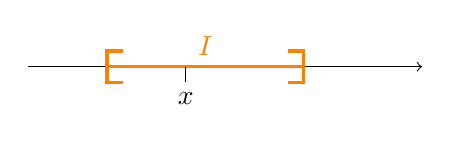
\begin{tikzpicture}
			\draw[->] (0,0) -- (5,0);
			\draw[very thick,orange] (1,0) -- node[midway,above] {$I$} (3.5,0)
			(1.2,0.2) -- (1,0.2) -- (1,-0.2) -- (1.2,-0.2)
			(3.3,0.2) -- (3.5,0.2) -- (3.5,-0.2) -- (3.3,-0.2)
			;
			\draw (2,0) -- ++(0,-0.2) node[below] {$x$};
		\end{tikzpicture}
	\end{minipage}
	\begin{minipage}{0.4\linewidth}
		On note	\squareFrame{$x ∈ I$}.
	\end{minipage}
\end{frame}

\begin{frame}
	Un \textbf{ensemble} est ainsi une collection d'éléments.

	\pause
	\vspace{1.5em}
	\begin{minipage}{0.5\linewidth}
		\begin{tikzpicture}
			\draw (0,0) ellipse (2.5 and 1.7);
			\node at (-1.8,1.5) {$E$};
			\coordinate (e₁) at (-1,0.8);
			\coordinate (e₂) at (1,-0.5);
			\coordinate (e₃) at (-0.6,-0.7);
			\foreach \x in {e₁,e₂,e₃} {
					\node at (\x) {×};
					\node[above] at (\x) {$\x$};
				}
		\end{tikzpicture}
	\end{minipage}
	\begin{minipage}{0.4\linewidth}
		On note	\squareFrame{$E = \Big\{e₁,e₂,e₃\Big\}$}.
	\end{minipage}
\end{frame}

\begin{frame}
	\begin{center}
		\begin{tikzpicture}
			\draw<1>[red!0] (3,0) ellipse (2.5 and 1.7);
			\draw<1>[fill=red!50] (0,0) ellipse (2.5 and 1.7);
			\draw<2>[blue!0] (0,0) ellipse (2.5 and 1.7);
			\draw<2>[fill=blue!50] (3,0) ellipse (2.5 and 1.7);
			\begin{scope}[even odd rule]
				\clip<3,4> (0,0) ellipse (2.5 and 1.7);
				\draw<3,4>[fill=violet!50] (3,0) ellipse (2.5 and 1.7);
			\end{scope}
			\draw<5,6>[fill=orange!50] (0,0) ellipse (2.5 and 1.7);
			\draw<5,6>[fill=orange!50] (3,0) ellipse (2.5 and 1.7);
			\node<1,3->[red!70] at (-1.9,1.5) {$E₁$};
			\node<2,3->[blue!70] at (4.8,1.5) {$E₂$};
			\coordinate (e₁) at (-1,0);
			\coordinate (e₂) at (4,0);
			\coordinate (e₃) at (1.5,0);
			\foreach \x in {e₁,e₂,e₃} {
					\node<7-> at (\x) {×};
					\node<7->[above] at (\x) {$\x$};
				}
			\draw (0,0) ellipse (2.5 and 1.7);
			\draw (3,0) ellipse (2.5 and 1.7);
		\end{tikzpicture}
	\end{center}

	\vspace{2em}
	\only<4>{$$E₁ ∩ E₂$$}
	\only<6>{$$E₁ ∪ E₂$$}
	\only<8>{
		$$ e₁ ∈ E₁ ∪ E₂ \hspace{2em} e₂ ∈ E₁ ∪ E₂ \hspace{2em} e₃ ∈ E₁ ∪ E₂ $$
	}
	\only<9>{
		$$ e₃ ∈ E₁ ∩ E₂ $$
	}
\end{frame}

\begin{frame}
	\begin{center}
		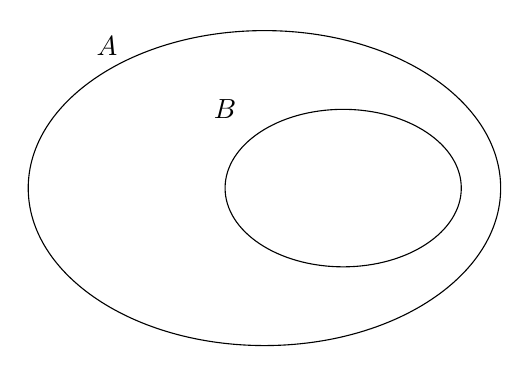
\begin{tikzpicture}
			\draw (0,0) ellipse (3 and 2);
			\draw (1,0) ellipse (1.5 and 1);
			\node at (-2,1.8) {$A$};
			\node at (-0.5,1) {$B$};
		\end{tikzpicture}

		\pause
		$$B ⊂ A$$
	\end{center}
\end{frame}

\begin{frame}
	\begin{center}
		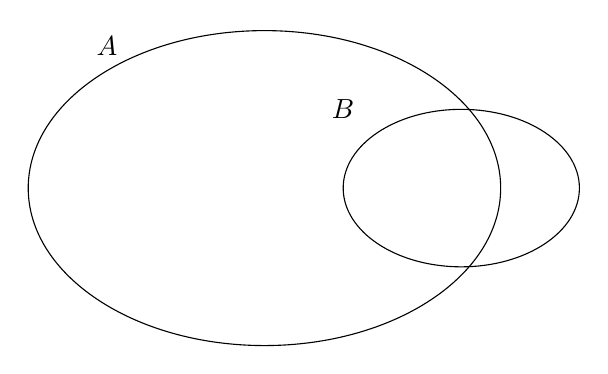
\begin{tikzpicture}
			\draw (0,0) ellipse (3 and 2);
			\draw (2.5,0) ellipse (1.5 and 1);
			\node at (-2,1.8) {$A$};
			\node at (1,1) {$B$};
		\end{tikzpicture}

		\pause
		$$B \not⊂ A$$
	\end{center}
\end{frame}

\end{document}